\subsubsection{Server - OrderGateway}
\begin{figure}[H]
	\centering
%	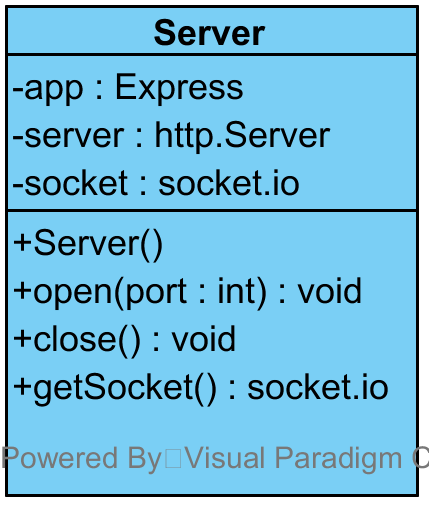
\includegraphics[width=15cm]{./diagrammi/demo/server.png}
	\caption{Componente OrderGateway}
\end{figure}
Il server è composto dall'OrderGateway, che ne è la base, dal package Order, che contiene le classi che rappresentano degli ordini, e da Menu, il quale fornisce e gestisce varie operazioni.

\setclass{BubbleAndEat::OrderGateway::OrderGateway}
\paragraph[::OrderGateway]{\class}\mbox{}\\ \label{\class}
\begin{figure}[H]
	\centering
%	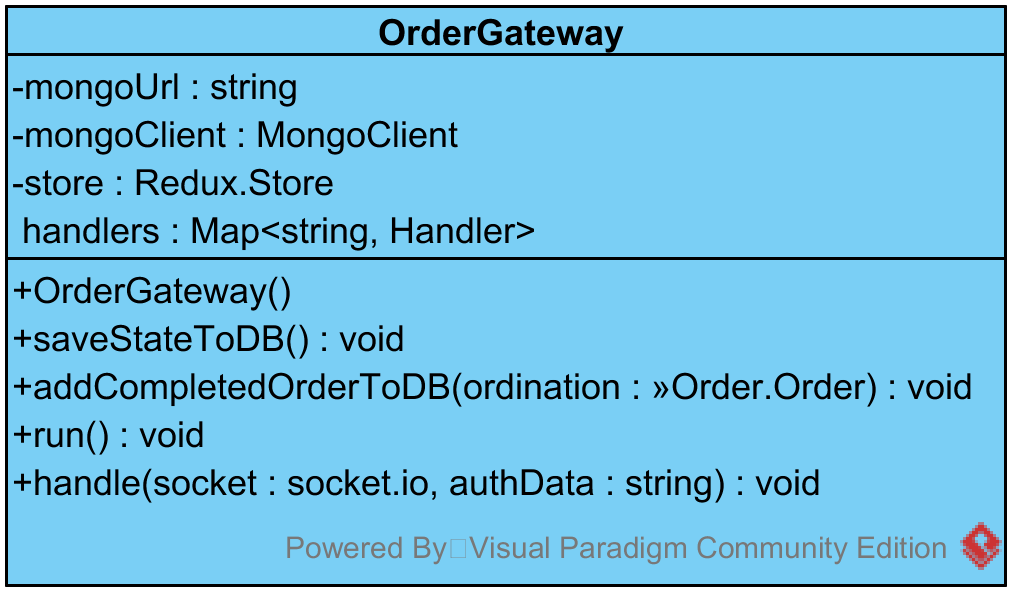
\includegraphics[width=7cm]{./diagrammi/demo/server/ordergateway.png}
	\caption{Classe \class}
\end{figure}
\textbf{Descrizione:}\\
Classe che rappresenta un gateway per le comunicazioni tra le bubble e il server.

\textbf{Utilizzo:}\\
Viene utilizzata per inizializzare le connessioni e indirizzare le comunicazioni alle giuste bubble attraverso appositi handler.

%\textbf{Classi ereditate:}
%\begin{itemize}
%	\item \code{}.
%\end{itemize}
%
%\textbf{Sottoclassi:}
%\begin{itemize}
%	\item \coderef{}.
%\end{itemize}

\textbf{Attributi:}
\begin{itemize}
	\item \field{- mongoClient: MongoClient}: database MongoDB;
	\item \field{- mongoUrl: string}: URI del database;
	\item \field{- store: Redux::Store}: oggetto contenente lo stato dell'applicazione.
\end{itemize}

\textbf{Metodi:}
\begin{itemize}
	\item \method{+ OrderGateway()}: costruttore, inizializza lo stato dell'applicazione recuperandolo, se possibile, dal database;
	\item \method{+ saveStatetoDB(): void}: effettua la connessione al database e salva lo stato dell'applicazione;
	\item \method{+ addCompletedOrderToDB(ordination: Order): void}: aggiunge l'ordine alla collezione degli ordini completati sul database:
	\begin{itemize}
		\item \param{ordination: Order}: l'ordine completato da aggiungere;
	\end{itemize}
	\item \method{+ run(): void}: avvia il server;
	\item \method{+ handler(socket: Socket.Io): void}: gestisce le connessioni indirizzandole al corretto handler.
\end{itemize}


\setclass{BubbleAndEat::OrderGateway::MenuItem}
\paragraph[::MenuItem]{\class}\mbox{}\\ \label{\class}
\begin{figure}[H]
	\centering
	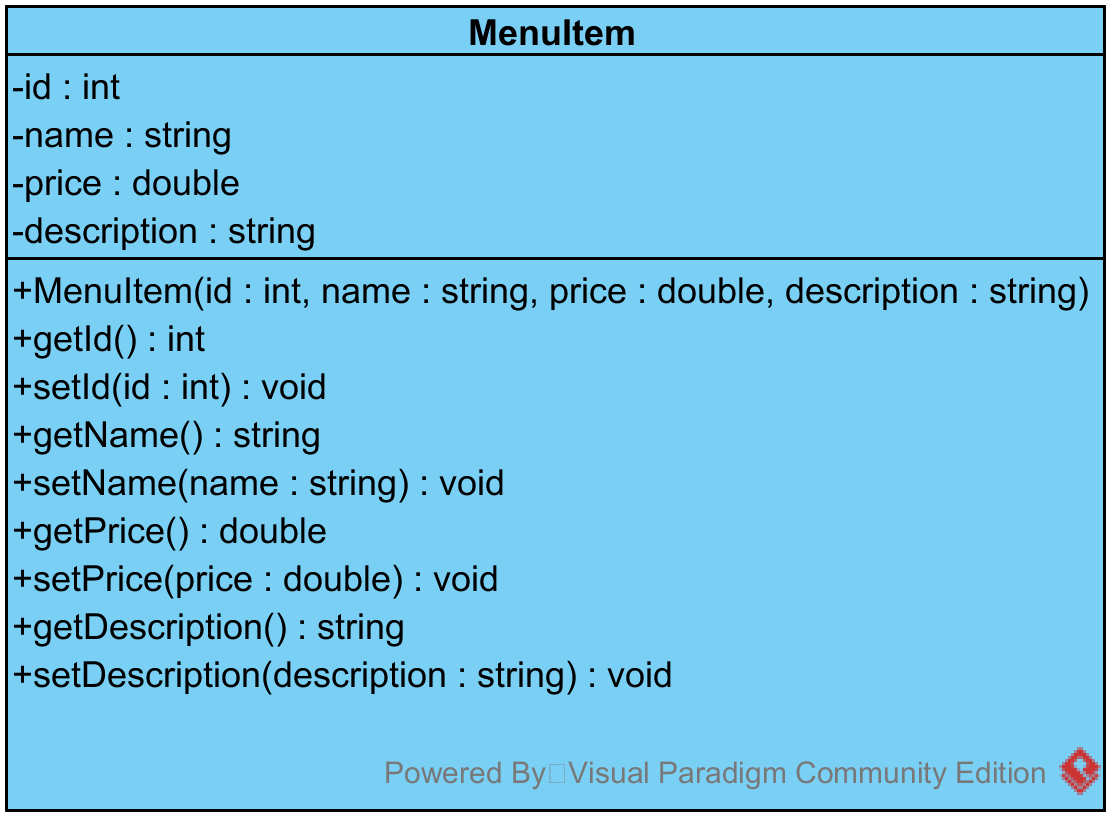
\includegraphics[width=10cm]{./diagrammi/demo/server/menuitem.png}
	\caption{Classe \class}
\end{figure}
\textbf{Descrizione:}\\
Classe che rappresenta una singola voce del menu.

\textbf{Utilizzo:}\\
Viene utilizzata per creare le singole pietanze da mostrare nel menu e da inserire negli ordini.

%\textbf{Classi ereditate:}
%\begin{itemize}
%	\item \code{}.
%\end{itemize}
%
%\textbf{Sottoclassi:}
%\begin{itemize}
%	\item \coderef{}.
%\end{itemize}

\textbf{Attributi:}
\begin{itemize}
	\item \field{- id: int}: numero identificativo della pietanza del menu;
	\item \field{- name: string}: nome della pietanza;
	\item \field{- price: double}: prezzo della pietanza;
	\item \field{- description: string}: descrizione della pietanza.
\end{itemize}

\textbf{Metodi:}
\begin{itemize}
	\item \method{+ MenuItem(id: int, name: string, price: double, description: string)}: costruttore, assegna i parametri ai corrispondenti attributi:
	\begin{itemize}
		\item \param{id: int}: id della pietanza;
		\item \param{name: string}: nome della pietanza;
		\item \param{price: double}: prezzo della pietanza;
		\item \param{description: string}: descrizione della pietanza;
	\end{itemize}
	\item \method{+ getId(): int} getter per \texttt{id};
	\item \method{+ setId(id: int): void}: setter per \texttt{id};
	\item \method{+ getName(): string} getter per \texttt{name};
	\item \method{+ setName(name: string): void}: setter per \texttt{name};
	\item \method{+ getPrice(): double} getter per \texttt{price};
	\item \method{+ setPrice(price: double): void}: setter per \texttt{price};
	\item \method{+ getDescription(): string} getter per \texttt{description};
	\item \method{+ setDesctiption(description: string): void}: setter per \texttt{description};
\end{itemize}

\setclass{BubbleAndEat::OrderGateway::Menu}
\paragraph[::Menu]{\class}\mbox{}\\ \label{\class}
\begin{figure}[H]
	\centering
	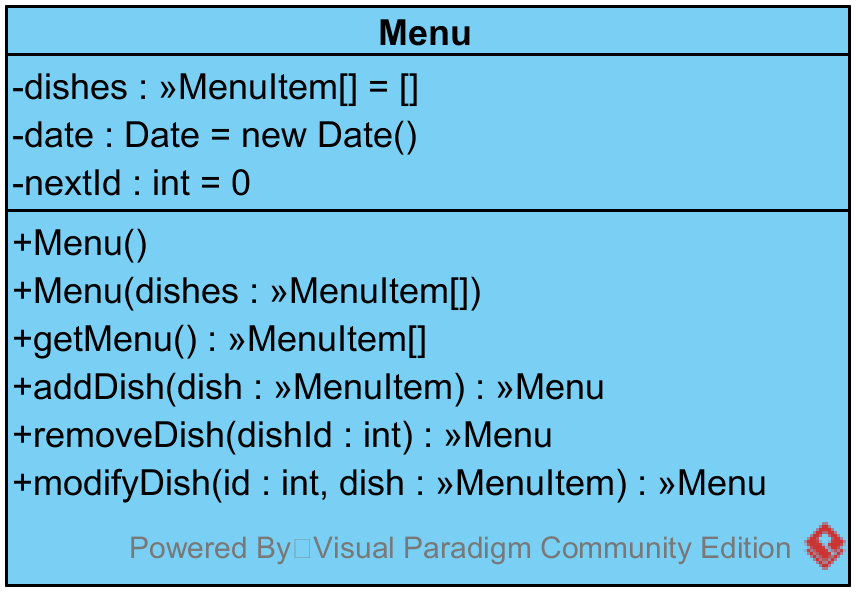
\includegraphics[width=8cm]{./diagrammi/demo/server/menu.png}
	\caption{Classe \class}
\end{figure}
\textbf{Descrizione:}\\
Classe che rappresenta il menu.

\textbf{Utilizzo:}\\
Viene utilizzata per raccogliere e gestire le pietanze disponibili nel ristorante.

%\textbf{Classi ereditate:}
%\begin{itemize}
%	\item \code{}.
%\end{itemize}
%
%\textbf{Sottoclassi:}
%\begin{itemize}
%	\item \coderef{}.
%\end{itemize}

\textbf{Attributi:}
\begin{itemize}
	\item \field{- dishes: MenuItem[] = []}: array contenete le pietanze del menu;
	\item \field{- date: Date = new Date()}: data di creazione del menu;
	\item \field{- nextId: int = 0}: numero di pietanze inserite e id per la nuova pietanza da inserire.
\end{itemize}

\textbf{Metodi:}
\begin{itemize}
	\item \method{+ Menu()}: costruttore di default;
	\item \method{+ Menu(dishes: MenuItem[])}: costruttore, inizializza l'array delle pietanze:
	\begin{itemize}
		\item \param{dishes: MenuItem[]}: array di pietanze;
	\end{itemize}
	\item \method{+ getMenu(): MenuItem[]} getter per \texttt{dishes};
	\item \method{+ addDish(dish: MenuItem): Menu}: permette di aggiungere una pietanza al menu:
	\begin{itemize}
		\item \param{dish: Menuitem}: pietanza da aggiungere
	\end{itemize}
	\item \method{+ removeDish(dishId: int): Menu} rimuove la pietanza con id \texttt{dishId} dal menu:
	\begin{itemize}
		\item \param{dishId: int}: id della pietanza da rimuovere;
	\end{itemize}
	\item \method{+ modifyDish(id: int, dish: MenuItem): Menu}: modifica la pietanza con id \texttt{id} in \texttt{dish}:
	\begin{itemize}
		\item \param{id: int}: id della pietanza da modificare;
		\item \param{dish: MenuItem}: pietanza con informazioni aggiornate.
	\end{itemize}
\end{itemize}

\setclass{BubbleAndEat::OrderGateway::Order}
\paragraph[::Order]{\class}\mbox{}\\ \label{\class}
\begin{figure}[H]
	\centering
	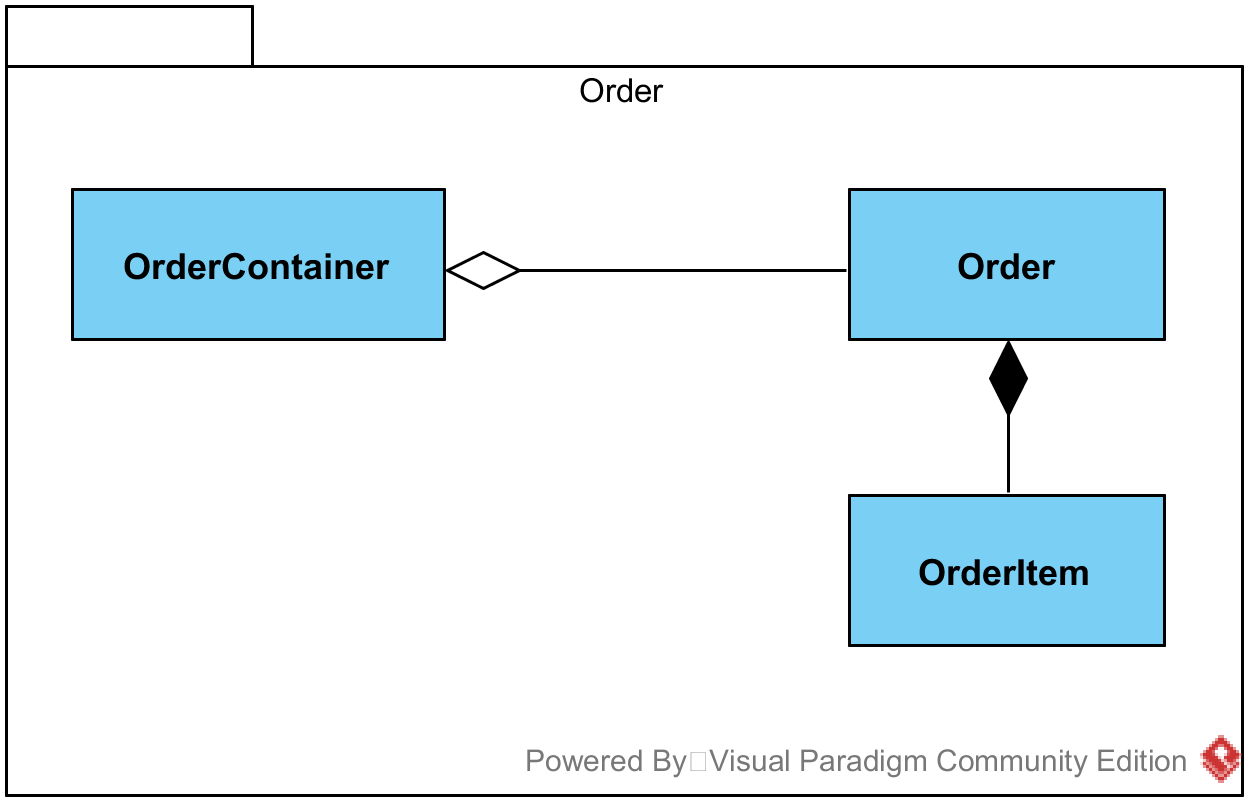
\includegraphics[width=12cm]{./diagrammi/demo/server/orderpkg.png}
	\caption{Componente \class}
\end{figure}

Questo componente ha la funzione di rappresentare gli ordini.

\setclass{BubbleAndEat::OrderGateway::Order::OrderContainer}
\subparagraph[::OrderContainer]{\class}\mbox{}\\ \label{\class}
\begin{figure}[H]
	\centering
	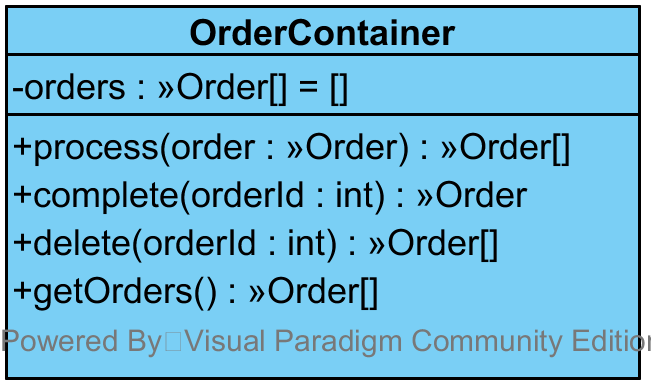
\includegraphics[width=7cm]{./diagrammi/demo/server/order/ordercontainer.png}
	\caption{Classe \class}
\end{figure}
\textbf{Descrizione:}\\
Classe che rappresenta un contenitore per gli ordini.

\textbf{Utilizzo:}\\
Viene utilizzata come contenitore comune degli ordini attivi per tutti gli utenti interni al ristorante.

%\textbf{Classi ereditate:}
%\begin{itemize}
%	\item \code{}.
%\end{itemize}
%
%\textbf{Sottoclassi:}
%\begin{itemize}
%	\item \coderef{}.
%\end{itemize}

\textbf{Attributi:}
\begin{itemize}
	\item \field{- \ul{orders: Order[] = []}}: array contenente gli ordini, inizializzato di default ad un array vuoto. È statico in quanto la lista degli ordini è condivisa da tutte le bubble.
\end{itemize}

\textbf{Metodi:}
\begin{itemize}
	\item \method{+ process(order: Order): Order[]}: processa l'ordine, lo imposta come attivo e lo aggiunge all'array \texttt{orders}:
	\begin{itemize}
		\item \param{order: Order}: il nuovo ordine da processare;
	\end{itemize}
	\item \method{+ complete(orderId: int): Order}: l'ordine con id \texttt{orderId} viene completato e il suo stato aggiornato;
	\item \method{+ delete(orderId: int): Order[]}: l'ordine con id \texttt{orderId} viene eliminato dalla lista degli ordini attivi.
\end{itemize}

\setclass{BubbleAndEat::OrderGateway::Order::Order}
\subparagraph[::Order]{\class}\mbox{}\\ \label{\class}
\begin{figure}[H]
	\centering
	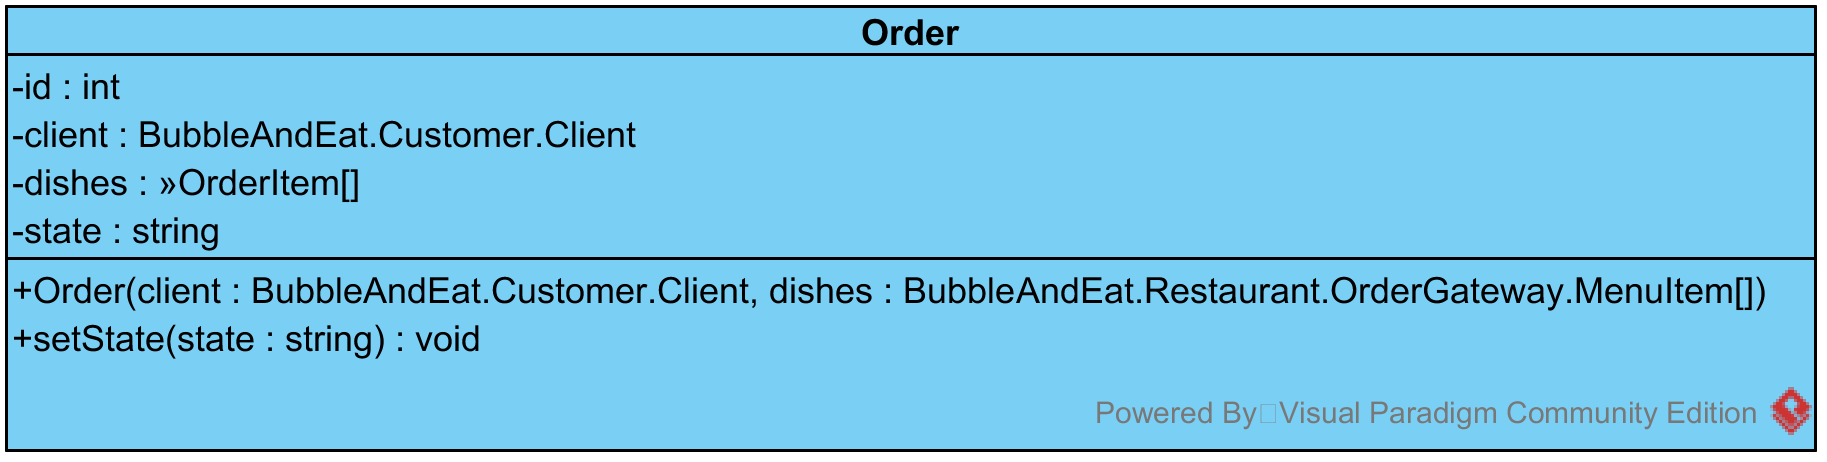
\includegraphics[width=15cm]{./diagrammi/demo/server/order/order.png}
	\caption{Classe \class}
\end{figure}
\textbf{Descrizione:}\\
Classe che rappresenta un singolo ordine.

\textbf{Utilizzo:}\\
Viene utilizzata per rappresentare i singoli ordini effettuati dai clienti, ovvero l'insieme delle pietanze che un utente ha ordinato.

%\textbf{Classi ereditate:}
%\begin{itemize}
%	\item \code{}.
%\end{itemize}
%
%\textbf{Sottoclassi:}
%\begin{itemize}
%	\item \coderef{}.
%\end{itemize}

\textbf{Attributi:}
\begin{itemize}
	\item \field{- id: int}: numero identificativo dell'ordine;
	\item \field{- client: Client}: cliente che ha effettuato l'ordine;
	\item \field{- dishes: OrderItem[]}: lista dei piatti ordinati;
	\item \field{- state: string}: indica lo stato di avanzamento dell'ordine.
\end{itemize}

\textbf{Metodi:}
\begin{itemize}
	\item \method{+ Order(client: Client, dishes: OrderItem[])}: costruttore, crea un nuovo ordine con cliente e pietanze ordinate:
	\begin{itemize}
		\item \param{client: Client}: cliente che ha effettuato l'ordine;
		\item \param{dishes: MenuItem[]}: pietanze ordinate;
	\end{itemize}
	\item \method{+ setState(state: string): void}: permette di aggiornare lo stato dell'ordine.
\end{itemize}

\setclass{BubbleAndEat::OrderGateway::OrderItem}
\subparagraph[::OrderItem]{\class}\mbox{}\\ \label{\class}
\begin{figure}[H]
	\centering
	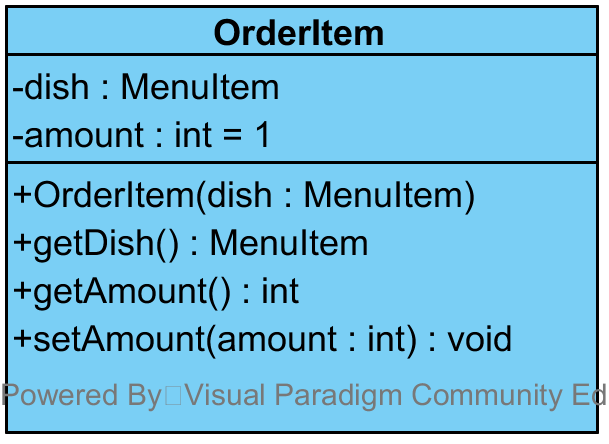
\includegraphics[width=12cm]{./diagrammi/demo/server/order/orderitem.png}
	\caption{Classe \class}
\end{figure}
\textbf{Descrizione:}\\
Classe che rappresenta una pietanza dell'ordine.

\textbf{Utilizzo:}\\
Viene utilizzata per memorizzare le quantità per ogni singolo piatto incluso nell'ordine.

%\textbf{Classi ereditate:}
%\begin{itemize}
%	\item \code{}.
%\end{itemize}
%
%\textbf{Sottoclassi:}
%\begin{itemize}
%	\item \coderef{}.
%\end{itemize}

\textbf{Attributi:}
\begin{itemize}
	\item \field{- dish: MenuItem}: piatto selezionato dal menu;
	\item \field{- amount: int = 1}: quantità selezionata (di default vale 1, altrimenti la voce dell'ordine non ha senso di esistere).
\end{itemize}

\textbf{Metodi:}
\begin{itemize}
	\item \method{+ OrderItem(dish: MenuItem)}: costruttore della classe, crea una voce dell'ordine per la pietanza \emph{dish};
	\item \method{+ getDish(): MenuItem}: getter per \texttt{dish};
	\item \method{+ getAmount(): int}: getter per \texttt{amount};
	\item \method{+ setAmount(amount: int): void}: setter per \texttt{amount}.
\end{itemize}